%% abtex2-modelo-relatorio-tecnico.tex, v-1.9.6 laurocesar
%% Copyright 2012-2016 by abnTeX2 group at http://www.abntex.net.br/ 
%%
%% This work may be distributed and/or modified under the
%% conditions of the LaTeX Project Public License, either version 1.3
%% of this license or (at your option) any later version.
%% The latest version of this license is in
%%   http://www.latex-project.org/lppl.txt
%% and version 1.3 or later is part of all distributions of LaTeX
%% version 2005/12/01 or later.
%%
%% This work has the LPPL maintenance status `maintained'.
%% 
%% The Current Maintainer of this work is the abnTeX2 team, led
%% by Lauro César Araujo. Further information are available on 
%% http://www.abntex.net.br/
%%
%% This work consists of the files abntex2-modelo-relatorio-tecnico.tex,
%% abntex2-modelo-include-comandos and abntex2-modelo-references.bib
%%

% ------------------------------------------------------------------------
% ------------------------------------------------------------------------
% abnTeX2: Modelo de Relatório Técnico/Acadêmico em conformidade com 
% ABNT NBR 10719:2015 Informação e documentação - Relatório técnico e/ou
% científico - Apresentação
% ------------------------------------------------------------------------ 
% ------------------------------------------------------------------------

\documentclass[
	% -- opções da classe memoir --
	12pt,				% tamanho da fonte
	article,			% não quebra páginas em novos capitulos
	openright,			% capítulos começam em pág ímpar (insere página vazia caso preciso)
	%twoside,			% para impressão em recto e verso. Oposto a oneside
	oneside,
	a4paper,			% tamanho do papel. 
	% -- opções da classe abntex2 --
	chapter=TITLE,		% títulos de capítulos convertidos em letras maiúsculas
	section=TITLE,		% títulos de seções convertidos em letras maiúsculas
	%subsection=TITLE,	% títulos de subseções convertidos em letras maiúsculas
	%subsubsection=TITLE,% títulos de subsubseções convertidos em letras maiúsculas
	% -- opções do pacote babel --
	english,			% idioma adicional para hifenização
	french,				% idioma adicional para hifenização
	spanish,			% idioma adicional para hifenização
	brazil,				% o último idioma é o principal do documento
]{abntex2}


% ---
% PACOTES
% ---

% ---
% Pacotes fundamentais 
% ---
\usepackage{lmodern}			% Usa a fonte Latin Modern
\usepackage[T1]{fontenc}		% Selecao de codigos de fonte.
\usepackage[utf8]{inputenc}		% Codificacao do documento (conversão automática dos acentos)
\usepackage{indentfirst}		% Indenta o primeiro parágrafo de cada seção.
\usepackage{color}				% Controle das cores
\usepackage{graphicx}			% Inclusão de gráficos
\usepackage{microtype} 			% para melhorias de justificação
% ---

% ---
% Pacotes adicionais, usados no anexo do modelo de folha de identificação
% ---
\usepackage{multicol}
\usepackage{multirow}
% ---

% ---
% Pacotes adicionais
% ---
\usepackage{placeins}	% permite usar 
\usepackage{wrapfig} % Permite textos em volta de figuras
\usepackage{pdfpages} % Permite usar o \includepdf
% ---

% ---
% Pacotes de citações
% ---
\usepackage[brazilian,hyperpageref]{backref}	 % Paginas com as citações na bibl
\usepackage[alf]{abntex2cite}	% Citações padrão ABNT

% ---
% Pacotes de códigos fonte
% ---
\usepackage{listingsutf8}

% Pacote para desenho de blocos
\usepackage{schemabloc}
\usetikzlibrary{circuits, arrows.meta, decorations.markings}

% ref: http://www.texample.net/tikz/examples/double-arrows/
\tikzstyle{innerWhite} = [thick, double distance=4, -{Triangle[open, scale=0.5]}, postaction={draw, line width=1mm, white, shorten >=2mm, -}]

% Para matrizes:
\usepackage{amsmath} 

% --- 
% CONFIGURAÇÕES DE PACOTES
% --- 

% ---
% Configurações do pacote backref
% Usado sem a opção hyperpageref de backref
\renewcommand{\backrefpagesname}{Citado na(s) página(s):~}
% Texto padrão antes do número das páginas
\renewcommand{\backref}{}
% Define os textos da citação
\renewcommand*{\backrefalt}[4]{
%	\ifcase #1 %
%	Nenhuma citação no texto.%
%	\or
%	Citado na página #2.%
%	\else
%	Citado #1 vezes nas páginas #2.%
%	\fi
}%
% ---

% ---
% Informações de dados para CAPA e FOLHA DE ROSTO
% ---
\titulo{PROJETO E IMPLEMENTAÇÃO DE CONTROLADOR DIGITAL NO ESPAÇO DE ESTADOS}
\autor{João Antônio Cardoso}
\local{Florianópolis}
\data{\today}
%\data{2015, v-1.9.6}
\orientador[Prof. ]{Flábio Alberto Bardemaker Batista}
\instituicao{Instituto Federal de Educação, Ciência e Tecnologia de Santa Catarina - Campus Florianópolis \\
	Engenharia Eletrônica \\
	Sistemas de Controle II
}
\tipotrabalho{Relatório técnico}
% O preambulo deve conter o tipo do trabalho, o objetivo, 
% o nome da instituição e a área de concentração 
\preambulo{\@title - relatório técnico para aprovação na parte laboratorial da disciplina de Sistemas de Controle II.}
% ---

% ---
% Configurações de aparência do PDF final

% alterando o aspecto da cor azul
\definecolor{blue}{RGB}{41,5,195}

% informações do PDF
\makeatletter
\hypersetup{
	pdftitle={\@title},
	pdfauthor={\@author},
	pdfsubject={\imprimirpreambulo},
	pdfcreator={LaTeX},
	colorlinks=true,       		% false: boxed links; true: colored links
	linkcolor=blue,          	% color of internal links
	citecolor=blue,        		% color of links to bibliography
	filecolor=magenta,      	% color of file links
	urlcolor=blue
}
\makeatother
% --- 

% ---
% Modificando a capa padrão
% ---
\renewcommand{\imprimircapa}{
	\begin{capa}
		\SingleSpacing
		\begin{adjustwidth}{}{}			
			\begin{minipage}{1\textwidth}
				\begin{wrapfigure}{l}{0.25\textwidth}
					\vspace*{-1em}\includegraphics[height=4em]{logotipo_ifsc.jpg}
				\end{wrapfigure}
				\imprimirinstituicao 
			\end{minipage}
			\vfill
			\begin{center}\ABNTEXchapterfont\LARGE\imprimirtitulo
				\vfill
				\small
				\begin{center}
					Aluno: \imprimirautor\\[1em]
					\imprimirorientadorRotulo\imprimirorientador\\
					\imprimircoorientadorRotulo\imprimircoorientador
				\end{center}
				\vfill
				\imprimirlocal, \imprimirdata
			\end{center}	
		\end{adjustwidth}
	\end{capa}
}

% --- 
% Espaçamentos entre linhas e parágrafos 
% --- 

% O tamanho do parágrafo é dado por:
\setlength{\parindent}{1.3cm}

% Controle do espaçamento entre um parágrafo e outro:
\setlength{\parskip}{0.2cm}  % tente também \onelineskip

% ---
% compila o indice
% ---
\makeindex
% ---

% ----
% Início do documento
% ----
\begin{document}
	
	% Seleciona o idioma do documento (conforme pacotes do babel)
	%\selectlanguage{english}
	\selectlanguage{brazil}
	
	% Retira espaço extra obsoleto entre as frases.
	\frenchspacing 
	
	% ----------------------------------------------------------
	% ELEMENTOS PRÉ-TEXTUAIS
	% ----------------------------------------------------------
	% \pretextual
	
	% ---
	% Capa
	% ---
	\imprimircapa
	% ---
	
	% ---
	% inserir o sumario
	% ---
	\pdfbookmark[0]{\contentsname}{toc}
	\tableofcontents*
	%\cleardoublepage
	% ---
	
	% ---
	% inserir lista de figuras
	% ---
	\clearpage
	\listoffigures
	\vspace{34pt}
	\listoftables
	
	% ----------------------------------------------------------
	% ELEMENTOS TEXTUAIS
	% ----------------------------------------------------------
	\textual
	
	\pagebreak
	
	% ----------------------------------------------------------
	% Introdução (exemplo de capítulo sem numeração, mas presente no Sumário)
	% ----------------------------------------------------------
	\chapter*[Introdução]{Introdução}
	\addcontentsline{toc}{chapter}{Introdução}
	
    Este trabalho apresenta um relatório do processo de solução do primeiro trabalho da disciplina de Sistemas de Controle II, no qual se pretende projetar e implementar um controlador digital, da teoria à prática laboratorial.
	
	\section[Objetivos]{Objetivos}
	
	A partir de um enunciado explicando a proposta de trabalho disponibilizada pelo professor, o autor propõe os seguintes itens como objetivos deste trabalho:
	
	\begin{itemize}
	    \item Fabricar uma planta para ser controlada.
	    \item Identificar a função de transferência equivalente da planta.
	    \item Especificar os requisitos do projeto.
	    \item Modelar a planta no espaço de estados.
	    \item Projetar um controlador no espaço de estados.
	    \item Projetar um observador de ordem mínima no espaço de estados.
	    \item Simular o sistema controlado e observador utilizando equações recursivas.
	    \item Implementar o controlador e observador em um \textit{microcontrolador}.
	    \item Avaliar o funcionamento da solução implementada.
		\item (opção do autor) Desenvolver o projeto utilizando somente softwares gratuitos, respeitando suas licenças de uso, dando preferência para softwares de código aberto.
	\end{itemize}
	
	\section[Desenvolvimento]{Desenvolvimento}

    	Como objeto de estudo, uma planta para ser controlada foi proposta pelo professor, e modificada de acordo com a disponibilidade de componentes e também modificada para a utilização de alimentação simples ao invés de alimentação simétrica, facilitando a montagem, que desta forma pode ocorrer diretamente por uma porta USB 1.0, comum em nossas ferramentas de trabalho como osciloscópios e computadores.
    	
    	Por se tratar de um projeto de controle digital, o autor optou por utilizar um \textit{DSP} \textit{TMS320F28335} da \textit{Texas Instruments} como controlador, imbutido em um \textit{Control Card}, conectado à um kit de desenvolvimento chamado \textit{C2000 Peripheral Explorer Kit}.
    	
    	\subsection{Modelagem da Planta}
    	
        	A planta resultante (\autoref{fig-planta}) consiste em três nós que são interconectados por meio de dois blocos. O bloco entre os nós \textbf{A} e \textbf{B} pode ser compreendido como um filtro passa-baixa de primeira ordem ativo de ganho unitário. O segundo bloco, entre os nós \textbf{B} e \textbf{C}, pode ser compreendido como um filtro passa-baixa de segunda ordem ativo de ganho unitário, utilizando uma topologia conhecida como \textit{Sallen-key}. 
        	
        	\begin{figure}[htbp]
        		\centering
        		\caption{Planta}
        		\includegraphics[width=\textwidth,height=240px,keepaspectratio]{imgs/planta.png}
        		\label{fig-planta}
        		\legend{Fonte: do autor. }
        	\end{figure}
        	
        	A partir do esquemático da planta (\autoref{fig-planta}), um novo esquemático foi desenhado no software de projeto de placas de circuito impresso \textit{KiCAD}, contendo pontos de teste, conectores e \textit{jumpers} para facilitar o teste dos blocos isoladamente. Para tal esquemático, \textit{layout} foi desenhado, e a placa manufaturada.
        	
        	Como o amplificador operacional do primeiro bloco fornece a característica de alta impedância na entrada e baixa impedância na saída, podemos caracterizar os dois blocos separadamente. Sendo assim, as equações no espaço de estados para o bloco 1 pode ser vista em \ref{eq-ssb1} e do segundo bloco, na \ref{eq-ssb2}.
        	
        	\begin{eqnarray}
        		\nonumber
                \dot{x_1} = 
                \begin{bmatrix}
                    \frac{-1}{R_3 C_3}
                \end{bmatrix}x_1
                +
                \begin{bmatrix}
                    0 \\
                    \frac{1}{R_3 C_3}
                \end{bmatrix}u_1 \\
                \label{eq-ssb1}
                    y_1 = 
                \begin{bmatrix}
                    1 \\
                \end{bmatrix}x_1
                +
                \begin{bmatrix}
                    0 \\
                \end{bmatrix}u_1
            \end{eqnarray}
            \begin{eqnarray}
        		\nonumber
        		\dot{x_2} = 
                \begin{bmatrix}
                    0 & \frac{1}{R_2 C_1} \\
                    \frac{-1}{R_1 C_2} & -\left( \frac{1}{R_1 C_2} + \frac{1}{R_2 C_2} \right)
                \end{bmatrix}x_2
                +
                \begin{bmatrix}
                    0 \\
                    \frac{1}{R_1 C_2}
                \end{bmatrix}u_2 \\
                \label{eq-ssb2}
                y_2 = 
                \begin{bmatrix}
                    1 & 0 \\
                \end{bmatrix}x_2
                +
                \begin{bmatrix}
                    0
                \end{bmatrix}u_2
        	\end{eqnarray}
        	
        	Para modelar o sistema completo podemos conectar as saídas do primeiro bloco nas entradas do segundo bloco e re-arranjar as matrizes de estados para obtermos um sistema equivalente, conforme explicado por \citeonline{lanari}, chegamos em \ref{eq-ssplanta_pre}:
        	
        	\begin{eqnarray}
        	    \nonumber
        		\dot{x} = 
                \begin{bmatrix}
                    \frac{-1}{R_3 C_3} & 0 & 0 \\
                    0 & 0 & \frac{1}{R_2 C_1} \\
                    \frac{1}{R_1 C_2} & \frac{-1}{R_1 C_2} & -\left( \frac{1}{R_1 C_2} + \frac{1}{R_2 C_2} \right) \\
                \end{bmatrix}x
                +
                \begin{bmatrix}
                    \frac{1}{R_3 C_3} \\
                    0 \\
                    0 \\
                \end{bmatrix}u \\
                \label{eq-ssplanta_pre}
                y = 
                \begin{bmatrix}
                    0 & 1 & 0 \\
                \end{bmatrix}x
                +
                \begin{bmatrix}
                    0
                \end{bmatrix}u
        	\end{eqnarray}
        	
        	Reorganizando nossa matriz para facilitar a utilização da metodologia do observador de estados de ordem mínima, mantendo o estado $x_1$ como nosso estado a ser medido (e não observado) $v_{C_1}$, e também para ficar mais intuitivo, podemos fazer o estado $x_2$ coincidir com $v_{C_2}$ e $x_3$ com $v_{C_3}$. Para tal, podemos trocar as posições da primeira e terceira linhas/colunas de todas as matrizes e consequentemente trocar as posições da primeira e e segunda, ficando com \ref{eq-ssplanta}:
        	
        	\begin{eqnarray}
        	    \nonumber
                \dot{x} = 
                \begin{bmatrix}
                    \dot{x_1} \\
                    \dot{x_2} \\
                    \dot{x_3} \\
                \end{bmatrix} = 
                \begin{bmatrix}
                    \dot{v_{C_1}} \\
                    \dot{v_{C_2}} \\
                    \dot{v_{C_3}} \\
                \end{bmatrix} =
                \overbrace{
                    \begin{bmatrix}
                        0 & \frac{1}{R_2 C_1} & 0 \\
                        \frac{-1}{R_1 C_2} & -\left( \frac{1}{R_1 C_2} + \frac{1}{R_2 C_2} \right) & \frac{1}{R_1 C_2} \\
                        0 & 0 & \frac{-1}{R_3 C_3}
                    \end{bmatrix}}^{A} x
                +
                \overbrace{
                    \begin{bmatrix}
                        0 \\
                        0 \\
                        \frac{1}{R_3 C_3}
                    \end{bmatrix}}^{B} u \\
                \label{eq-ssplanta}
                y = 
                \overbrace{
                    \begin{bmatrix}
                        1 & 0 & 0 \\
                    \end{bmatrix}}^{C} x
                +
                \overbrace{
                    \begin{bmatrix}
                        0
                    \end{bmatrix}}^{D} u
            \end{eqnarray}
        	
        	Como projetar um controlador que funcione para toda a gama de tolerância dos componentes está fora do contexto desta disciplina, vamos projetar um controlador considerando apenas os valores nominais dos componentes, resultando em \ref{eq-ssplanta_final}:
        	
        	\begin{eqnarray}
        	    \nonumber
                \dot{x} = 
                \begin{bmatrix}
                    \dot{x_1} \\
                    \dot{x_2} \\
                    \dot{x_3} \\
                \end{bmatrix} = 
                \begin{bmatrix}
                    \dot{v_{C_1}} \\
                    \dot{v_{C_2}} \\
                    \dot{v_{C_3}} \\
                \end{bmatrix} =
                \overbrace{
                    \begin{bmatrix}
                        0 & 559.44 & 0 \\
                        -21.01 & -100.93 & 21.01 \\
                        0 & 0 & -666.67
                    \end{bmatrix}}^{A} x
                +
                \overbrace{
                    \begin{bmatrix}
                        0 \\
                        0 \\
                        666.67
                    \end{bmatrix}}^{B} u \\
                \label{eq-ssplanta_final}
                y = 
                \overbrace{
                    \begin{bmatrix}
                        1 & 0 & 0 \\
                    \end{bmatrix}}^{C} x
                +
                \overbrace{
                    \begin{bmatrix}
                        0
                    \end{bmatrix}}^{D} u
            \end{eqnarray}
            
        \subsubsection{Resposta ao degrau da planta modelada}
        
        Utilizando um software de simulação matemática podemos aplicar um sinal arbitrário na entrada de nosso espaço de estados com uma entrada e uma saída (\textit{SISO}) e plotar todos os seus estados, além de sua entrada e saída, conforme a \autoref{fig-step_response_openloop}:
        
        \begin{figure}[htbp]
        	\centering
        	\caption{Resposta ao Degrau da Planta Modelada}
        	\includegraphics[width=\textwidth,height=240px,keepaspectratio]{imgs/step_response_openloop.png}
        	\label{fig-step_response_openloop}
        	\legend{Fonte: do autor. }
    	\end{figure}
    	
    	Podemos também realizar uma simulação para o sistema em malha aberto resolvendo as equações do espaço de estados da planta modelada recursivamente, obtendo a \autoref{fig-step_response_recursive_openloop}, no qual pode ser percebida a grande semelhança entre as saídas realizadas na simulação utilizando a função \textit{control.forced\_response()}, aqui chamada de \textit{lsim}, por ser equivalente à função do \textit{MATLAB}.
    	
    	\begin{figure}[htbp]
        	\centering
        	\caption{Resposta ao Degrau da Planta Modelada - Implementação Recursiva}
        	\includegraphics[width=\textwidth,height=240px,keepaspectratio]{imgs/step_response_recursive_openloop.png}
        	\label{fig-step_response_recursive_openloop}
        	\legend{Fonte: do autor. }
    	\end{figure}
    	
    	\subsection{Identificação da Planta}
    	
        	Uma técnica para a identificação da planta pode ser aplicar um sinal conhecido e a partir de figuras de mérito, levantar seus parâmetros e equacionar uma função de transferência de segundo grau equivalente.
        	
        	Por se tratar de uma planta que trabalha em uma região de tensão positiva na entrada e saída, e também por sabermos que o circuito possui não linearidades próximo aos valores de sua alimentação, aqui iremos aplicar um degrau de 1 à $1.5\,[V]$, ou seja, não é um degrau unitário, mas é um sinal conhecido e tomando alguns cuidados, toda a teoria que utiliza degraus unitários pode ser utilizada.
        	
        	Para deixar explícito como foram computadas as figuras de mérito, as Equações \ref{eq-mp} à \ref{eq-settling_time} descrevem o modo com que foram calculados os valores de \textit{Tempo de Subida} (\textit{Rise Time} - $t_r$) \textit{Sobressinal} (\textit{Overshoot} - $Mp$), o \textit{Tempo de Acomodação em 5\%} (Settling Time - $t_{s_{5\%}}$ ).
        	
        	\begin{eqnarray}
        		\nonumber
        		V_{10\%} = 0,1\cdot(\;V_{\infty} -V_{0}\;) \\
        		\nonumber
        		V_{90\%} = 0,9\cdot(\;V_{\infty} -V_{0}\;) \\
        		\label{eq-mp}
        		t_{r} = t_{(V_{90\%})} - t_{(V_{10\%})} \\
        		\nonumber
        		V_{max_{5\%}} \leq (1 +0.05) \cdot (V_{(\infty)} - V_{0}) +V_{0} \\
        		\nonumber
        		V_{min_{5\%}} \leq (1 -0,05) \cdot (V_{(\infty)} - V_{0}) +V_{0} \\
        		\label{eq-settling_time}
        		t_{s_{5\%}} = max\left(\; t_{(Vmax_{5\%})}\quad, \quad t_{(Vmin_{5\%})}\;\right)		
        	\end{eqnarray}
        	
        	Antes de realizar as medições, a primeira etapa foi executar a auto-calibração do osciloscópio e calibrar manualmente as ponteiras, para garantir que não houvessem erros técnicos nas medições.
        	
        	Com o osciloscópio devidamente calibrado, verificou-se o sinal \textit{PWM} de entrada, se estava na frequência de operação correta, e se estava nos ciclos-tarefa como foi calculado. 
        	
        	O gatilho do osciloscópio foi configurado no canal 2, que mostra o momento em que o degrau é aplicado, portanto, todas as medidas de tempo com os cursores são relativos ao tempo em que o degrau foi aplicado, que será considerado como o tempo inicial ($t_0=0\,[s]$).
        	
        	A primeira ponteira do osciloscópio foi então conectada na saída da planta. O resultado é mostrado na \autoref{fig-ftma-step}.
        	
        	Para medir com maior precisão, optou-se por trabalhar com o diferentes escalas do osciloscópio para focar em cada parte da forma de onda. A fim de alcançar uma precisão ainda melhor no osciloscópio, foi utilizado o \textit{trigger} no \textit{modo normal}, que permitiu que a função de média de 128 amostras na aquisição atuasse como uma sobre-amostragem, adicionando pelo menos três bits de precisão no desenho da forma de onda, reduzindo consideravelmente o ruído aleatório.
        	
        	Para que o relatório não fique demasiadamente longo, as capturas do osciloscópio detalhadas para cada aquisição de tempo de subida, tempo de acomodação e tempo de pico constam no \autoref{ap-ftma} para a planta completa em malha aberta.
    	
    	\subsection{Planta em Malha Aberta}
        
            Podemos considerar a planta em malha aberta como uma \textit{caixa preta} e obter suas figuras de mérito aplicando um sinal arbitrário em sua entrada.
            
            \begin{figure}[htbp]
            	\centering
            	\caption{Resposta ao Degrau na Planta em Malha Aberta}
            	\includegraphics[width=\textwidth,height=240px,keepaspectratio]{imgs/ftma/step_response.JPG}
            	\label{fig-ftma-step}
            	\legend{Resposta ao degrau de $0,5\,[V]$ aplicado pela tensão média do \textit{PWM}. No Canal 1 (Amarelo) é a saída da planta e o canal 2 (azul), o \textit{trigger}. Fonte: do autor. }
        	\end{figure}
            
            No \ref{ap-ftma} pode ser verificado a captura para a obtenção dos parâmetros, que foram:
            \FloatBarrier
                $$V_{0}=0\,[V]$$
                $$V_{\infty}=1,49\,[V]$$
                $$t_{subida}=15,0\,[ms]$$
                $$t_{50\%}=12,0\,[ms]$$
                $$t_{s5\%}=47,6\,[ms]$$
                $$V_{pk}=1.57\,[V]$$
                $$t_{pk}=34,0\,[ms]$$
                $$M_{p}=16,3265\%$$
                $$\zeta = 0,4997062 $$
                $$w_n = 103,330164 [rad/s]$$
            \FloatBarrier
            
            Tendo a planta caracterizada, precisamos definir nossos requisitos de projeto.
        
        \subsection{Requisitos de Projeto}
        
            Como objetivo do projeto, o professor propôs um controlador que modifique o \textit{Tempo de Acomodação de 5\%} e o \textit{Sobressinal} para a metade de seus valores em malha aberta, ou seja, neste caso ficamos com $t_{s5\%}\leq25,4\,[ms]$ e $M_{p}\leq8,05\%$. Outra exigência é que haja erro nulo em regime permanente e que o sistema controlado seja estável.

        \subsection{Projeto do Controlador}
        
            A topologia para o sistema em malha fechada utilizada aqui é de um controlador de servossistema com a inserção de um integrador, como mostrado em \autoref{fig-planta-blocos-sem-obs}.
            
            \begin{figure}[htbp]
                \centering
                \caption{Diagrama de blocos do projeto de servossistemas sem observador}
                \label{fig-planta-blocos-sem-obs}
                \resizebox{\textwidth}{!}{
                    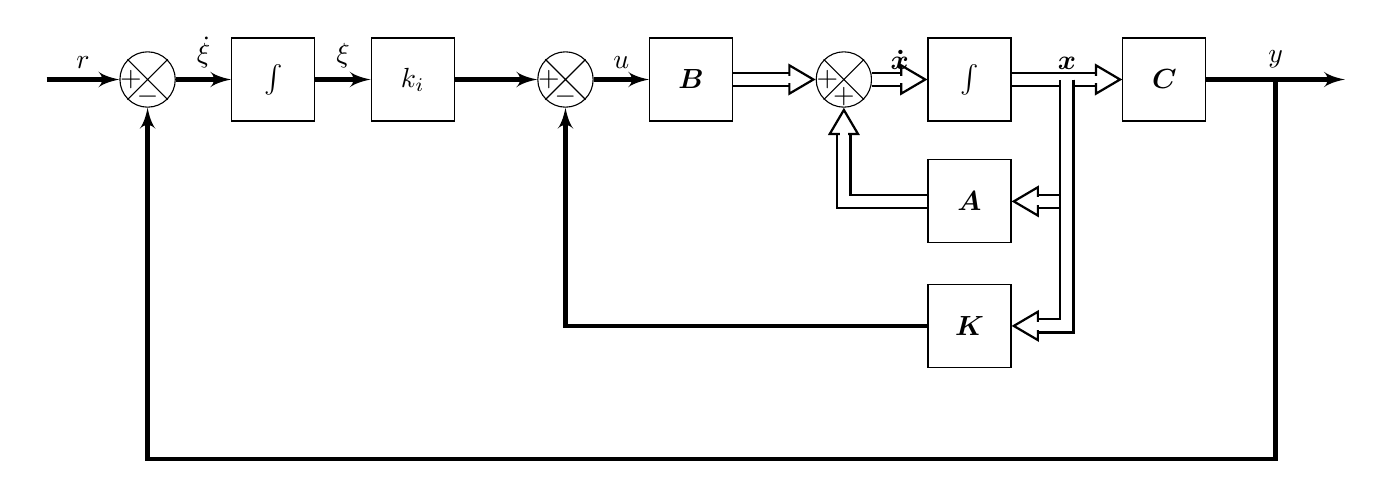
\begin{tikzpicture}
                        \sbStyleLien{ultra thick}
                        \sbEntree{in}
                        \sbComp{comp_in_out}{in}
                        \sbRelier[$r$]{in}{comp_in_out}
                        
                        \sbBloc{int_xi}{$\int$}{comp_in_out}
                        \sbRelier[$\dot{\xi}$]{comp_in_out}{int_xi}
                        
                        \sbBloc{ki}{$k_i$}{int_xi}
                        \sbRelier[$\xi$]{int_xi}{ki}
                        
                        \sbComp{comp_ki_K}{ki}
                        \sbRelier[$ $]{ki}{comp_ki_K}
                        
                        \sbBloc{B}{$\boldsymbol{B}$}{comp_ki_K}
                        \sbRelier[$u$]{comp_ki_K}{B}
                        
                        \sbStyleLienDefaut
                        \sbStyleLien{innerWhite}
                        \sbSumb{comp_Ax_Bu}{B}
                        \sbRelier[$ $]{B}{comp_Ax_Bu}
                        
                        \sbBloc{int_x}{$\boldsymbol{\int}$}{comp_Ax_Bu}
                        \sbRelier[$\boldsymbol{\dot{x}}$]{comp_Ax_Bu}{int_x}
                        
                        \sbBloc[4]{C}{$\boldsymbol{C}$}{int_x}
                        \sbRelier[$\boldsymbol{x}$]{int_x}{C}
                        
                        \sbDecaleNoeudy{int_x-C}{_A}
                        \sbBlocr{A}{$\boldsymbol{A}$}{_A}
                        \sbRelieryx{int_x-C}{A}
                        \sbRelierxy{A}{comp_Ax_Bu}
                        
                        \sbDecaleNoeudy[9.5]{int_x-C}{_K}
                        \sbBlocr{K}{$\boldsymbol{K}$}{_K}
                        \sbRelieryx{int_x-C}{K}
                        
                        \sbStyleLienDefaut
                        \sbStyleLien{ultra thick}
                        
                        \sbRelierxy{K}{comp_ki_K}
                        
                        \sbSortie[5]{out}{C}
                        \sbRelier[$y$]{C}{out}
                        \sbRenvoi[13]{C-out}{comp_in_out}{}
                    \end{tikzpicture}
                }
                \legend{Fonte: do autor. }
            \end{figure}
            
            Para alcançar os requisito de projeto, precisamos definir a localização dos polos dominantes quando fecharmos a malha. 
            
            Para tal, pode-se utilizar uma relação analítica aproximada entre as figuras de mérito de um sistema de segunda ordem e os parâmetros de um sistema de segundo grau conhecidos como fator de amortecimento ($\zeta$) e frequência natural ($w_n$). É importante salientar que são aproximações e que ao utilizarmos essas equações estamos admitindo uma margem de erro nos resultados do projeto, e também, que serão necessários quatro polos para o sistema e a localização dos dois polos não dominantes pode influenciar drasticamente nos resultados.
            
            O projetista escreveu uma rotina em \textit{Python} que variava a posição dos polos não dominantes seguindo algumas estratégias de posicionamento, testava o resultado dos sistemas (\autoref{fig-strategies_comparison} e selecionava o de menor sobressinal, resultando nos seguintes polos para o projeto do controlador conforme \ref{eq-polos-controlador}, que foram posicionados utilizando o segundo e terceiro polos como um par complexo conjugado, reduzindo o valor de sua parte imaginária por um fator ampliando a parte real para seu dobro. Na \autoref{fig-strategies_comparison} a estratégia escolhida é mostrada como \textit{Estratégia [54]}, tendo um $ \zeta $ de $0.7484$ e um $w_n$ de $158.1\,rad/s$, alcançando um sobressinal de $2.89\%$ e um tempo de acomodação de $22,4\,ms$.
            
            \begin{equation}
                \label{eq-polos-controlador}
                j = \begin{bmatrix}
                    -128.52101782 +171.08783376i & -128.52101782 -171.08783376i \\
                    -257.04203564  +1.71087834i & -257.04203564  -1.71087834i
                    \end{bmatrix}
            \end{equation}
            
            \begin{figure}[htbp]
            	\centering
            	\caption{Comparação das Estratégias de Posicionamentos dos Polos Não Dominantes}
            	\includegraphics[width=\textwidth,height=240px,keepaspectratio]{imgs/strategies_comparison.png}
            	\label{fig-strategies_comparison}
            	\legend{Comparação de resposta ao degrau dos sistemas controlados com o diferentes estratégias para o posicionamento dos polos não dominantes. Fonte: do autor. }
        	\end{figure}
            
            \subsubsection{Período de Integração para o Controlador}
            
                Como projetaremos um controlador digital, precisamos definir o período de integração que será empregado nos integradores do sistema. Para que o controlador alcance a resposta do sistema, consideramos aqui uma frequência de no mínimo duas vezes a frequência natural amortecida do sistema, que resultaria em aproximadamente $1320\,Hz$. 
                
                Neste ponto, o autor gostaria de deixar claro que houveram diversas iterações utilizando \textit{scripts} automatizados para projetar e testar o controle utilizando algumas taxas diferentes e chegou à conclusão que valores acima de $2kHz$ funcionavam bem, optando por ficar em \textbf{3kHz}. 
                
                Utilizando tal frequência para o integrador do controlador, temos um período aproximadamente 4,5 vezes menor que o período da frequência natural amortecida da planta.
                
            \subsubsection{Cálculo da Matriz de Ganhos do Controlador}
            
                Primeiramente verificamos se a nossa planta pode ser controlada verificando se sua matriz de controlabilidade tem o mesmo número de equações linearmente independentes que a quantidade de estados modelados. Para o sistema modelado o número de equações linearmente independentes coincide com seu número de estados, logo, é controlável.
            
                O controlador pode ser calculado a partir do método de \textit{Ackermann} para o sistema da \autoref{eq-acker-controlador} utilizando os polos definidos anteriormente em \autoref{eq-polos-controlador}, obtendo a matriz de ganhos do controlador \textbf{K}, mostrado na \autoref{eq-K}.
                
                \begin{equation}
                    \label{eq-acker-controlador}
                    \dot{e} = (\boldsymbol{\hat{A}} - \boldsymbol{\hat{B}}\,\boldsymbol{\hat{K}})\,e
                \end{equation}
                
                \begin{eqnarray}
                    \nonumber
                    \boldsymbol{\hat{A}} =
                    \begin{bmatrix}
                        \boldsymbol{A} & \boldsymbol{0} \\
                        \boldsymbol{-C} & 0
                    \end{bmatrix} = 
                    \begin{bmatrix}
                        0.           & 559.44055944  & 0.            & 0.        \\
                        -21.00840336 & -100.92848328 & 21.00840336   & 0.        \\
                        0.           & 0.            & -666.66666667 & 0.        \\
                        -1.          & 0.            & 0.            & 0.        \\
                    \end{bmatrix} \\
                    \nonumber
                    \boldsymbol{\hat{B}} =
                    \begin{bmatrix}
                        \boldsymbol{B} \\
                        0
                    \end{bmatrix}
                    \begin{bmatrix}
                        0.           \\
                        0.           \\
                        666.66666667 \\
                        0.           \\
                    \end{bmatrix} \\
                    \nonumber
                    \boldsymbol{\hat{C}} = 
                    \begin{bmatrix}
                        \boldsymbol{C} & 0.
                    \end{bmatrix} = 
                    \begin{bmatrix}
                        1. & 0. & 0. & 0.
                    \end{bmatrix} \\
                    \nonumber
                    \boldsymbol{\hat{D}} = \boldsymbol{D} = \begin{bmatrix} 0 \end{bmatrix} \\
                    \nonumber
                    \boldsymbol{\hat{K}} = \begin{bmatrix}
                        \boldsymbol{K} & -K_i
                    \end{bmatrix} \\
                    \label{eq-K}
                    \boldsymbol{K} = \begin{bmatrix}
                        4.16654212e+00 & 1.17530446e+01 & 5.29643546e-03
                    \end{bmatrix} \\
                    K_i = 386.12694507724626
                \end{eqnarray}
                
                Utilizando as matrizes de estados do sistema controlado $\boldsymbol{\hat{A}}$, $\boldsymbol{\hat{B}}$, $\boldsymbol{\hat{C}}$ e $\boldsymbol{\hat{D}}$ podemos simular o sistema controlado e também o sistema controlado amostrado na frequência de integração escolhida, como mostrado na \autoref{fig-step_response_closedloop}, coerente com sua implementação recursiva, que pode ser visto nas Figuras \ref{fig-step_response_recursive_closedloop} e \ref{fig-step_response_recursive_closedloop_zoom}.
                
                \begin{figure}[htbp]
                	\centering
                	\caption{Simulação com Controlador em Malha Fechada}
                	\includegraphics[width=\textwidth,height=240px,keepaspectratio]{imgs/step_response_closedloop.png}
                	\label{fig-step_response_closedloop}
                	\legend{Fonte: do autor. }
            	\end{figure}
            	
            	\begin{figure}[htbp]
                	\centering
                	\caption{Simulação com Controlador em Malha Fechada - Implementação Recursiva}
                	\includegraphics[width=\textwidth,height=240px,keepaspectratio]{imgs/step_response_recursive_closedloop.png}
                	\label{fig-step_response_recursive_closedloop}
                	\legend{Fonte: do autor. }
            	\end{figure}
            	
            	\begin{figure}[htbp]
                	\centering
                	\caption{Simulação com Controlador em Malha Fechada - Implementação Recursiva - Ampliado}
                	\includegraphics[width=\textwidth,height=240px,keepaspectratio]{imgs/step_response_recursive_closedloop_zoom.png}
                	\label{fig-step_response_recursive_closedloop_zoom}
                	\legend{Fonte: do autor. }
            	\end{figure}
                
            \subsection{Projeto do Observador}
            
                Para que seja possível obter os estados da planta sem a necessidade de implementar um sensor para cada um dos três estados, pode-se fazer o uso de um observador, que pode ser entendido como um modelo da planta simplificado do qual se utiliza para obter estimativas dos estados ($\boldsymbol{\tilde{x}}$) a partir de uma implementação realimentada. Aqui vamos utilizar um observador de ordem mínima, que no nosso caso, irá estimar os estados de $x_2$ e $x_3$ a partir da medição da saída $y$, que coincide com o estado $x_1$. A topologia do controlador de servossistema utilizando um observador pode ser visto na \autoref{fig-planta-blocos-com-obs}.
                
                \begin{figure}[htbp]
                    \centering
                    \caption{Diagrama de Blocos do Projeto de Servossistemas com Observador de Ordem Mínima}
                    \label{fig-planta-blocos-com-obs}
                    \resizebox{\textwidth}{!}{
                        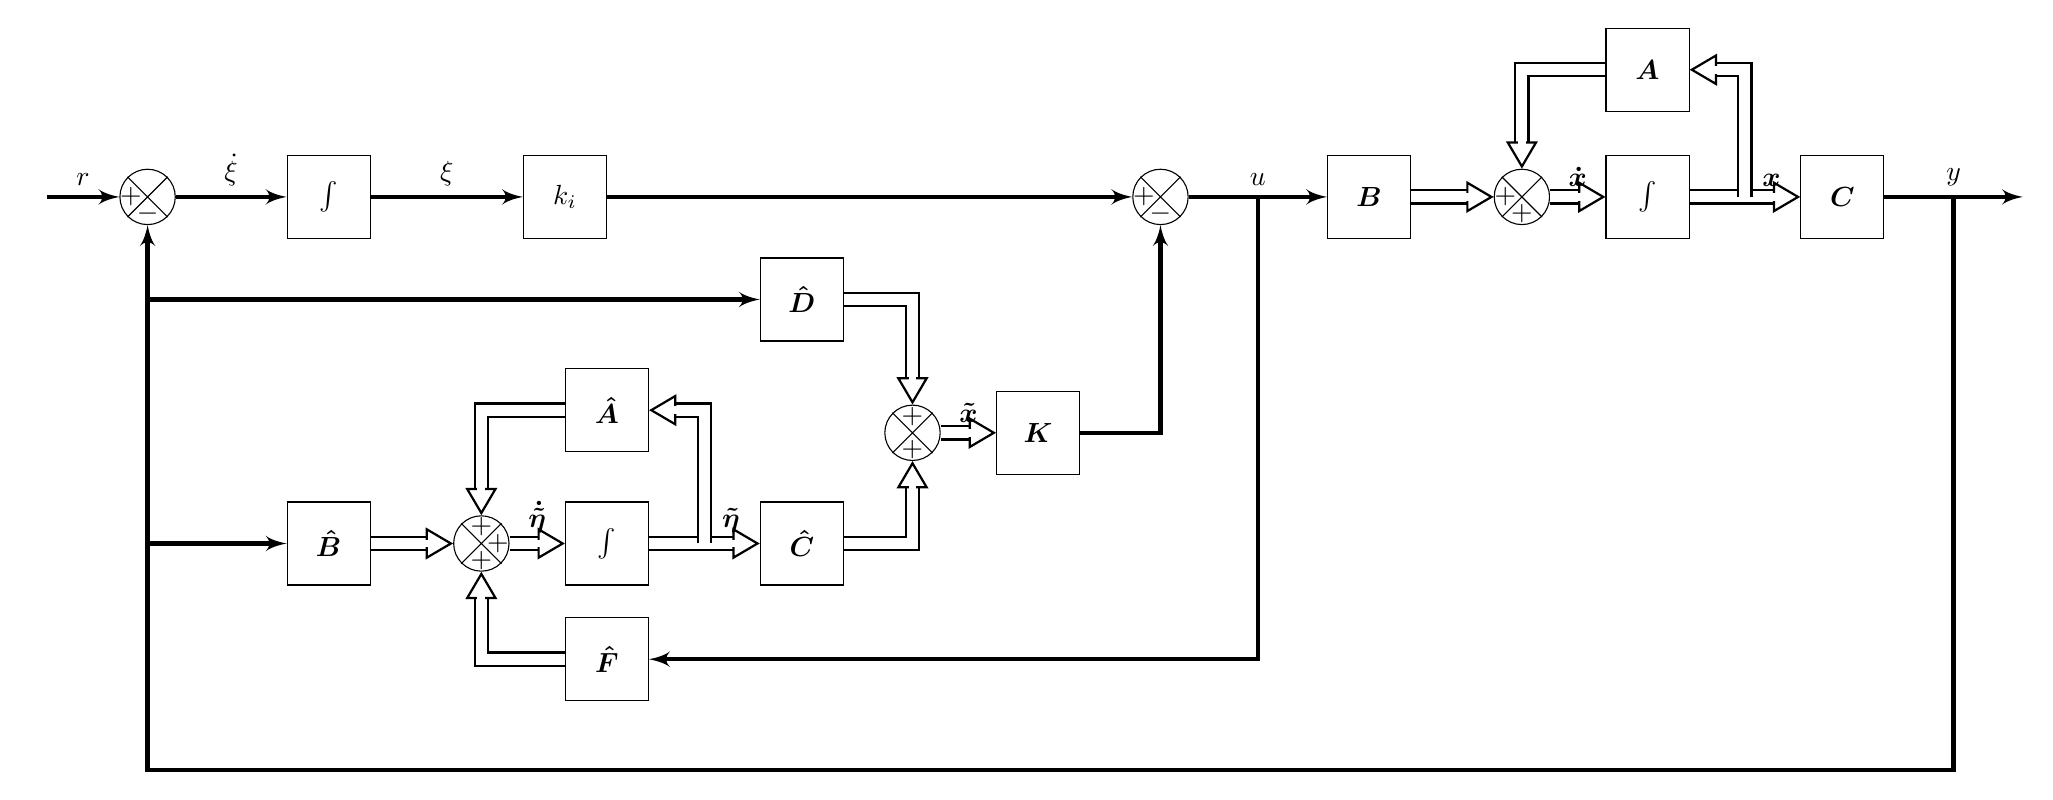
\begin{tikzpicture}
                        
                            \sbStyleLien{ultra thick}
                            
                            
                            \sbEntree{in}
                            \sbComp{comp_in_out}{in}
                            \sbRelier[$r$]{in}{comp_in_out}
                            
                            \sbBloc[4]{int_xi}{$\int$}{comp_in_out}
                            \sbRelier[$\dot{\xi}$]{comp_in_out}{int_xi}
                            
                            \sbBloc[5.5]{ki}{$k_i$}{int_xi}
                            \sbRelier[$\xi$]{int_xi}{ki}
                            
                            \sbComp[20]{comp_ki_K}{ki}
                            \sbRelier[$ $]{ki}{comp_ki_K}
                            
                            \sbBloc[5]{B}{$\boldsymbol{B}$}{comp_ki_K}
                            \sbRelier[$u$]{comp_ki_K}{B}
                            
                            
                            \sbStyleLienDefaut
                            \sbStyleLien{innerWhite}
                            
                            
                            \sbSumb{comp_Ax_Bu}{B}
                            \sbRelier[$ $]{B}{comp_Ax_Bu}
                            
                            \sbBloc{int_x}{$\boldsymbol{\int}$}{comp_Ax_Bu}
                            \sbRelier[$\boldsymbol{\dot{x}}$]{comp_Ax_Bu}{int_x}
                            
                            \sbBloc[4]{C}{$\boldsymbol{C}$}{int_x}
                            \sbRelier[$\boldsymbol{\,\,\,\,\,\,\,\,\,\,x}$]{int_x}{C}
                            
                            \sbDecaleNoeudy[-4]{int_x-C}{_A}
                            \sbBlocr{A}{$\boldsymbol{A}$}{_A}
                            \sbRelieryx{int_x-C}{A}
                            \sbRelierxy{A}{comp_Ax_Bu}
                            
                            
                            \sbStyleLienDefaut
                            \sbStyleLien{ultra thick}
                            
                            \sbSortie[5]{out}{C}
                            \sbRelier[$y$]{C}{out}
                            \sbRenvoi[20]{C-out}{comp_in_out}{}
                            
                            \sbDecaleNoeudy[13.5]{comp_in_out-int_xi}{_Bhat}
                            \sbDecaleNoeudy[1]{comp_in_out}{_out_feedback_node}
                            \sbBloc{Bhat}{$\boldsymbol{\hat{B}}$}{_Bhat}
                            \sbRelieryx{_out_feedback_node}{Bhat}
                            
                            
                            \sbStyleLienDefaut
                            \sbStyleLien{innerWhite}
                            
                            \sbCompSum{comp_Ahat_Bhat_Fhat}{Bhat}{+}{+}{ }{+}
                            
                            \sbRelier[$ $]{Bhat}{comp_Ahat_Bhat_Fhat}
                            
                            
                            \sbBloc{int_eta}{$\int$}{comp_Ahat_Bhat_Fhat}
                            \sbRelier[$\boldsymbol{\dot{\tilde{\eta}}}$]{comp_Ahat_Bhat_Fhat}{int_eta}
                            
                            \sbBloc[4]{Chat}{$\boldsymbol{\hat{C}}$}{int_eta}
                            \sbRelier[$\boldsymbol{\,\,\,\,\,\,\,\,\,\,\tilde{\eta}}$]{int_eta}{Chat}
                            
                            \sbDecaleNoeudy[-4]{int_eta-Chat}{_Ahat}
                            \sbBlocr{Ahat}{$\boldsymbol{\hat{A}}$}{_Ahat}
                            \sbRelieryx{int_eta-Chat}{Ahat}
                            \sbRelierxy{Ahat}{comp_Ahat_Bhat_Fhat}
                            
                            \sbStyleLienDefaut
                            \sbStyleLien{ultra thick}
                            
                            \sbDecaleNoeudy{int_eta-Chat}{_Fhat}
                            \sbBlocr{Fhat}{$\boldsymbol{\hat{F}}$}{_Fhat}
                            \sbRelieryx{comp_ki_K-B}{Fhat}
                            
                            \sbDecaleNoeudy[-8]{int_eta-Chat}{_Dhat}
                            \sbBloc{Dhat}{$\boldsymbol{\hat{D}}$}{_Dhat}
                            \sbRelieryx{_out_feedback_node}{Dhat}
                            
                            \sbDecaleNoeudy[-4]{Chat}{_Chat_Dhat}
                            \sbCompSum{comp_Chat_Dhat}{_Chat_Dhat}{+}{+}{ }{ }
                            
                            \sbBloc{K}{$\boldsymbol{K}$}{comp_Chat_Dhat}
                            
                            \sbRelierxy{K}{comp_ki_K}
                            
                            
                            \sbStyleLienDefaut
                            \sbStyleLien{innerWhite}
                            
                            \sbRelierxy{Chat}{comp_Chat_Dhat}
                            \sbRelierxy{Dhat}{comp_Chat_Dhat}
                            \sbRelier[$\boldsymbol{\tilde{x}}$]{comp_Chat_Dhat}{K}
                            
                            \sbRelierxy[$ $]{Fhat}{comp_Ahat_Bhat_Fhat}
                            
                        \end{tikzpicture}
                    }
                    \legend{Fonte: do autor. }
                \end{figure}
            
                Para que o observador consiga estimar os estados da planta controlada, podemos definir seus polos como o dobro da parte real dos polos dominantes do controlador, ficando com os polos mostrados na \autoref{eq-polos-observador}.
            
                \begin{equation}
                    \label{eq-polos-observador}
                    l = \begin{bmatrix}
                        -257.04203564 &-257.04203564
                        \end{bmatrix}
                \end{equation}
                
                O autor achou interessante utilizar um período de integração para o observador duas vezes menor que o período de integração do controlador, e ainda realizar uma sobre-amostragem, realizando 4 amostragens da variável de saída para cada observação de estados, criando assim, uma melhoria na precisão dos valores adquiridos.
            
            \subsubsection{Cálculo do Observador de Ordem Mínima}
            
                Primeiramente verificamos se a nossa planta pode ser observada verificando se sua matriz de observabilidade tem o mesmo número de equações linearmente independentes que a quantidade de estados modelados a serem observados. Para o sistema modelado o número de equações linearmente independentes coincide com seu número de estados -1, logo, é observável.
            
                O observador pode ser calculado a partir do método de \textit{Ackermann} para o sistema da \autoref{eq-acker-observador} utilizando os polos definidos anteriormente em \autoref{eq-polos-observador}, obtendo a matriz $\boldsymbol{K_e}$ e as matrizes de espaço de estados do observador $\boldsymbol{\hat{A}}$, $\boldsymbol{\hat{B}}$, $\boldsymbol{\hat{C}}$, $\boldsymbol{\hat{D}}$ e $\boldsymbol{\hat{F}}$.
                
                \begin{equation}
                    \label{eq-acker-observador}
                    \dot{e} = (\boldsymbol{{A_{bb}}'} - \boldsymbol{{K_e}}\,\boldsymbol{{A_{ab}}})'\,e
                \end{equation}
                
                \begin{eqnarray}
                    \nonumber
                    \boldsymbol{A} = 
                    \begin{bmatrix}
                        A_{aa} & A_{ab} \\
                        A_{ba} & A_{bb}
                    \end{bmatrix} \\
                    \nonumber
                    \boldsymbol{B} = 
                    \begin{bmatrix}
                        B_a & B_b \\
                    \end{bmatrix}
                \end{eqnarray}
                
                \begin{eqnarray}
                    \nonumber
                    A_{aa} = 0 \\
                    \nonumber
                    \boldsymbol{A_{ab}} = 
                    \begin{bmatrix}
                        559.44055944 &  0.
                    \end{bmatrix} \\
                    \nonumber
                    \boldsymbol{A_{b_a}} = 
                    \begin{bmatrix}
                        -21.00840336 \\
                        0.
                    \end{bmatrix} \\
                    \nonumber
                    \boldsymbol{A_{b_b}} =
                    \begin{bmatrix}
                        -100.92848328 & 21.00840336 \\
                        0.            & -666.66666667
                    \end{bmatrix} \\
                    \nonumber
                    Ba = 0 \\
                    \nonumber
                    \boldsymbol{B_b} = 
                    \begin{bmatrix}
                        0 \\
                        666.66666667
                    \end{bmatrix}
                \end{eqnarray}
                
                \begin{eqnarray}
                    \nonumber
                    \boldsymbol{\hat{A}} = \boldsymbol{A_{bb}} - \boldsymbol{K_e}\,\boldsymbol{A_{ab}} =
                    \begin{bmatrix}
                        152.58259539   &   21.00840336.  \\
                        -7986.91530517 & -666.66666667
                    \end{bmatrix} \\
                    \nonumber
                    \boldsymbol{\hat{B}} = \boldsymbol{\hat{A}}\,\boldsymbol{K_e} + \boldsymbol{A_{ba}} - \boldsymbol{K_e}\,A_{aa} =
                    \begin{bmatrix}
                        209.77743764    \\
                        -5898.46165694
                    \end{bmatrix} \\
                    \nonumber
                    \boldsymbol{\hat{C}} = 
                    \begin{bmatrix}
                        \boldsymbol{0} \\
                        \boldsymbol{I}.
                    \end{bmatrix} = 
                    \begin{bmatrix}
                        0. & 0.     \\
                        1. & 0.     \\
                        0. & 1.
                    \end{bmatrix} \\
                    \nonumber
                    \boldsymbol{\hat{D}} =
                    \begin{bmatrix}
                        0 \\
                        \boldsymbol{K_e}
                    \end{bmatrix} = 
                    \begin{bmatrix}
                        1. \\
                        -0.45315105 \\
                        14.27661111
                    \end{bmatrix} \\
                    \nonumber
                    \boldsymbol{\hat{F}} = \boldsymbol{B_b} - \boldsymbol{K_e}\,B_a = 
                    \begin{bmatrix}
                        0. \\
                        666.66666667
                    \end{bmatrix} \\
                    \label{eq-Ke}
                    \boldsymbol{K_e} = \begin{bmatrix}
                        -0.45315105 \\
                        14.27661111
                    \end{bmatrix}
                \end{eqnarray}
            
            \subsection{Simulação Completa - Implementação Recursiva}
            
                Utilizando as matrizes de estados da planta, a matriz de ganho do controlador e as matrizes de espaço de estados do observador podemos simular o sistema em recursividade para um sinal arbitrário e assim comparar os estados obtido através do observador e a partir da planta simulada através do comando \textit{control.forced\_response()}, que é equivalente ao \textit{lsim} do \textit{MATLAB}.
                
                Para melhorar a simulação, o autor considerou:
                \begin{itemize}
                    \item Quantização no ADC de 12 bits
                    \item Quantização no DAC de 12 bits
                    \item Frequência de integração do Observador em 6kHz
                    \item Frequência de integração do Controlador em 3kHz
                    \item Frequência de integração da planta (passo de simulação) em 50kHz
                    \item Ruído branco na saída planta de 100 mV
                \end{itemize}
                
                Os resultados gerais podem ser vistos na \autoref{fig-step_response_closedloop_observer} sem ruído, e na  \autoref{fig-step_response_closedloop_observer_noise}, com o ruído. 
                
                Figuras mais detalhadas com a comparação de cada estado do observador, assim como ampliação com detalhes nos degraus de subida e de descida, podem ser vistos no \autoref{ap-simul}.
                
                \FloatBarrier
                
                \begin{figure}[htbp]
                	\centering
                	\caption{Simulação com Controlador e Observador em Malha Fechada}
                	\includegraphics[width=\textwidth,height=240px,keepaspectratio]{imgs/step_response_closedloop_observer.png}
                	\label{fig-step_response_closedloop_observer}
                	\legend{Fonte: do autor. }
            	\end{figure}
            	
            	\begin{figure}[htbp]
                	\centering
                	\caption{Simulação com Controlador e Observador em Malha Fechada, com Ruído}
                	\includegraphics[width=\textwidth,height=240px,keepaspectratio]{imgs/step_response_closedloop_observer_noise.png}
                	\label{fig-step_response_closedloop_observer_noise}
                	\legend{Fonte: do autor. }
            	\end{figure}
            	
            	\FloatBarrier
            
            \subsubsection{Resultados}
            
                Um \textit{script}(\autoref{ap-scripts}) gerou as constantes utilizadas no \textit{firmware} implementado no \textit{DSP}. A resposta ao degrau para o sistema em malha fechada em comparação ao mesmo sistema em malha aberta pode ser visto na \autoref{fig-ftmf-step}.
                As formas de onda apresentam resultados similares aos esperados pela simulação da \autoref{fig-step_response_recursive_closedloop}.
                
                \begin{figure}[htbp]
                	\centering
                	\caption{Resposta ao Degrau na Planta em Malha Fechada e Aberta}
                	\includegraphics[width=\textwidth,height=240px,keepaspectratio]{imgs/ftmf/step_response.JPG}
                	\label{fig-ftmf-step}
                	\legend{Resposta ao degrau de $0,5\,[V]$ aplicado pela tensão média do \textit{PWM}. No Canal 1 (Amarelo) é a saída do sistema em malha fechada, o canal de referência A (Branco), representando a resposta ao degrau do sistema em malha aberta, e o canal 2 (azul), o \textit{trigger}. Fonte: do autor. }
            	\end{figure}
            	
            	O sinal da ação de controle \textbf{u} se manteve dentro dos valores de simulação, verificado através de ferramentas de \textit{debug} (entre 0,7 e 1,8 V).
            	
            	\FloatBarrier
                No \autoref{ap-ftmf} pode ser verificado a captura do osciloscópio para a obtenção de cada um dos parâmetros a seguir:
                $$V_{0}=1,0\,[V]$$
                $$V_{\infty}=1,5\,[V]$$
                $$t_{subida}=14,8\,[ms]$$
                $$t_{50\%}=13,6\,[ms]$$
                $$t_{s5\%}=23,8\,[ms]$$
                $$V_{pk}=1.51\,[V]$$
                $$t_{pk}=33,3\,[ms]$$
                $$M_{p}=2\%$$
                $$\zeta = 0.7797 $$
                $$w_n = 150.22 [rad/s]$$
                \FloatBarrier
                
                A \autoref{tab-resultados} apresenta uma comparação de todos os dados obtidos durante o processo.
                
                \begin{table}[htbp]
                    \label{tab-resultados}
                    \centering
                    \caption{Comparação dos resultados}
                    \begin{tabular}{r|c|c|c|c|c}
                                    &               $Mp\%$&     $t_{s5\%}[ms]$&     $t_r\,[ms]$ &       $v_{\inf}$ &	$v_{0}$ \\ \hline
                        Malha Aberta simulação  &   18,88 &     50,1 &              14,8 &              1,50 & 			1,00 \\
                        Malha Aberta prático  &     16,32 &     49,2 &              15,2 &              1,49 & 			1,01 \\
                        Malha Fechada simulação &   2,88 &      22,4 &              13,8 &              1,50 & 			1,00 \\
                        Malha Fechada prático &     2,00 &      23,8 &              14,8 &              1,50 &			1,00 \\
                        Requisitos	        &		8,05 &		25,0 &				N/A	&				N/A	&			N/A
                    \end{tabular}
                    \legend{Fonte: do autor.}
                \end{table}

    \section{Conclusões}
    
        Neste trabalho surgiram algumas dificuldades no âmbito algébrico, mas que foram aos poucos sendo superados com o decorrer do projeto.
        
        Para facilitar a implementação do projeto de controle no microcontrolador, o autor desenvolveu uma biblioteca em código aberto em $C 89$, utilizando somente macros, sendo compatível com a maior parte dos microcontroladores, possibilitando a descrição matemática do sistema facilmente seguindo o fluxo dos diagramas de blocos. Alguns outros trabalhos de colegas também tiveram sucesso ao utilizarem esta implementação em seus projetos, então o autor considera que por facilitar não só este projeto, que foi um tempo bem investido.
        
        Neste projeto o autor optou por programar uma rotina que minimizasse os possíveis problemas causados pelos polos não dominantes do sistema, executando uma série de projetos de maneira automatizada, seguindo uma simples regra de seleção e o controlador que foi obtido se comportou de maneira estável.
        
        Os \textit{scripts} de simulação recursiva previram razoavelmente bem os resultados práticos, possibilitando uma série de iterações de testes e ajustes antes de propriamente implementar o controlador no microcontrolador.
        
        Além disso, o autor cumpriu seu objetivo pessoal de realizar o trabalho inteiramente com software gratuitos, inclusive o sistema operacional (\textit{Linux}), utilizando principalmente o \textit{KiCAD} para o projeto da placa de circuito impresso, o pacote de controle \textit{python-control} da linguagem de programação \textit{Python}, o qual inclusive contribuiu adicionando a funcionalidade \textit{stepinfo}, equivalente à função de mesmo nome do \textit{MATLAB}, e por fim o \textit{LaTeX} para compilação deste relatório.
     
        Deste modo, o autor considera este projeto um processo de grande valor para a formação do estudante de engenharia eletrônica, que em exercício, atua com a interface entre a informação teórica e o que é concebível com a tecnologia e recursos disponíveis.
    
    
	% ---
	% Finaliza a parte no bookmark do PDF
	% para que se inicie o bookmark na raiz
	% e adiciona espaço de parte no Sumário
	% ---
	\phantompart
	
	% ---
	% Conclusão
	% ---
	%\section[Conclusões e recomendações]{Conclusões e recomendações}
	% ---
	

	% ----------------------------------------------------------
	% ELEMENTOS PÓS-TEXTUAIS
	% ----------------------------------------------------------
	\postextual
	
	% ----------------------------------------------------------
	% Referências bibliográficas
	% ----------------------------------------------------------
	%\pagebreak
	\bibliography{main}
	
	% ----------------------------------------------------------
	% Glossário
	% ----------------------------------------------------------
	%
	% Consulte o manual da classe abntex2 para orientações sobre o glossário.
	%
	%\glossary
	
	% ----------------------------------------------------------
	% Apêndices
	% ----------------------------------------------------------
	
	% ---
	% Inicia os apêndices
	% ---
	\begin{apendicesenv}
	%	
	%	% Imprime uma página indicando o início dos apêndices
		\partapendices
	%	
% 		\chapter{questao1.m}
% 		\label{questao1.m}
% 		\lstinputlisting{questao1.m}
% 		\pagebreak
        \clearpage
	
    	\chapter{Resultados da Simulação Completa}
        	\label{ap-simul}
        	
        	\FloatBarrier
        	
        	\begin{figure}[htbp]
                	\centering
                	\caption{Simulação com Controlador e Observador em Malha Fechada}
                	\includegraphics[width=\textwidth,height=240px,keepaspectratio]{imgs/step_response_closedloop_observer_zoom_stepup.png}
                	\label{fig-step_response_closedloop_observer_zoom_stepup}
                	\legend{Fonte: do autor. }
        	\end{figure}
        	
        	\begin{figure}[htbp]
                	\centering
                	\caption{Simulação com Controlador e Observador em Malha Fechada}
                	\includegraphics[width=\textwidth,height=240px,keepaspectratio]{imgs/step_response_closedloop_observer_zoom_stepdown.png}
                	\label{fig-step_response_closedloop_observer_zoom_stepdown}
                	\legend{Fonte: do autor. }
        	\end{figure}
            	
        	\begin{figure}[htbp]
            	\centering
            	\caption{Simulação com Controlador e Observador em Malha Fechada - Estado 1}
            	\includegraphics[width=\textwidth,height=240px,keepaspectratio]{imgs/step_response_closedloop_observer_state1.png}
            	\label{fig-step_response_closedloop_observer_state1}
            	\legend{Fonte: do autor. }
        	\end{figure}
        	
        	\begin{figure}[htbp]
            	\centering
            	\caption{Simulação com Controlador e Observador em Malha Fechada - Estado 2}
            	\includegraphics[width=\textwidth,height=240px,keepaspectratio]{imgs/step_response_closedloop_observer_state2.png}
            	\label{fig-step_response_closedloop_observer_state2}
            	\legend{Fonte: do autor. }
        	\end{figure}
        	
        	\begin{figure}[htbp]
            	\centering
            	\caption{Simulação com Controlador e Observador em Malha Fechada - Estado 3}
            	\includegraphics[width=\textwidth,height=240px,keepaspectratio]{imgs/step_response_closedloop_observer_state3.png}
            	\label{fig-step_response_closedloop_observer_state3}
            	\legend{Fonte: do autor. }
        	\end{figure}
        	
        	\begin{figure}[htbp]
                	\centering
                	\caption{Simulação com Controlador e Observador em Malha Fechada, com Ruído}
                	\includegraphics[width=\textwidth,height=240px,keepaspectratio]{imgs/step_response_closedloop_observer_zoom_stepup_noise.png}
                	\label{fig-step_response_closedloop_observer_zoom_stepup_noise}
                	\legend{Fonte: do autor. }
        	\end{figure}
        	
        	\begin{figure}[htbp]
                	\centering
                	\caption{Simulação com Controlador e Observador em Malha Fechada, com Ruído}
                	\includegraphics[width=\textwidth,height=240px,keepaspectratio]{imgs/step_response_closedloop_observer_zoom_stepdown_noise.png}
                	\label{fig-step_response_closedloop_observer_zoom_stepdown_noise}
                	\legend{Fonte: do autor. }
        	\end{figure}
            	
        	\begin{figure}[htbp]
            	\centering
            	\caption{Simulação com Controlador e Observador em Malha Fechada - Estado 1, com Ruído}
            	\includegraphics[width=\textwidth,height=240px,keepaspectratio]{imgs/step_response_closedloop_observer_state1_noise.png}
            	\label{fig-step_response_closedloop_observer_state1_noise}
            	\legend{Fonte: do autor. }
        	\end{figure}
        	
        	\begin{figure}[htbp]
            	\centering
            	\caption{Simulação com Controlador e Observador em Malha Fechada - Estado 2, com Ruído}
            	\includegraphics[width=\textwidth,height=240px,keepaspectratio]{imgs/step_response_closedloop_observer_state2_noise.png}
            	\label{fig-step_response_closedloop_observer_state2_noise}
            	\legend{Fonte: do autor. }
        	\end{figure}
        	
        	\begin{figure}[htbp]
            	\centering
            	\caption{Simulação com Controlador e Observador em Malha Fechada - Estado 3, com Ruído}
            	\includegraphics[width=\textwidth,height=240px,keepaspectratio]{imgs/step_response_closedloop_observer_state3_noise.png}
            	\label{fig-step_response_closedloop_observer_state3_noise}
            	\legend{Fonte: do autor. }
        	\end{figure}
        	
        	\FloatBarrier
        	
    	\clearpage
        \chapter{Códigos Fonte do Projeto}
            \label{ap-scripts}
            Por somar mais de 50 páginas, o autor opta por não incluir a listagem dos códigos fonte no relatório, deixando todos  eles abertos em licença GPL3, disponíveis em um repositório público no \textit{github} do autor.
            
            Biblioteca desenvolvida para operações matriciais em C - C Arraay Macros:
            
            \url{https://github.com/joaoantoniocardoso/c_array_macros}
            
            Diretório raiz do repositório deste projeto de controle:
            
            \url{http://github.com/joaoantoniocardoso/sct2_projeto2}
            
            Para facilitar o acesso, o código fonte deste documento \textit{LaTeX} podem ser acessados em:
            
            \url{https://github.com/joaoantoniocardoso/sct2_projeto2/tree/master/tex}
            
            O código fonte do \textit{firmware} podem ser acessados em:
            
            \url{https://github.com/joaoantoniocardoso/sct2_projeto2/tree/master/f28335_ccs7/basic_F28335}
            
            O código fonte do \textit{hardware} podem ser acessados em:
            
            \url{https://github.com/joaoantoniocardoso/sct2_projeto2/tree/master/hardware/main}
            
            O código fonte para as simulações no \textit{LTSpice} podem ser acessados em:
            
            \url{https://github.com/joaoantoniocardoso/sct2_projeto2/tree/master/hardware/simulations}
            
            O código fonte dos \textit{scripts} em \textit{Python} e \textit{Jupyter Notebook} podem ser acessados em:
            
            \url{https://github.com/joaoantoniocardoso/sct2_projeto2/tree/master/controle}
            
            Por fim, o repositório pode ser baixado como um arquivo compactado em extensão \textit{.zip} em:
            
            \url{https://github.com/joaoantoniocardoso/sct2_projeto2/archive/master.zip}
            
        \clearpage
	
        \chapter{Capturas da Planta em Malha Aberta}
        	\label{ap-ftma}
        	
        	\FloatBarrier
        	\begin{figure}[htbp]
            	\centering
            	\caption{Tempo de Subida}
            	\includegraphics[width=\textwidth,height=240px,keepaspectratio]{imgs/ftma/rise_time.JPG}
            	\label{fig-ftma-rise_time}
            	\legend{Resposta ao degrau de $0,5\,[V]$ aplicado pela tensão média do \textit{PWM}. No Canal 1 (Amarelo) é a saída da planta e o canal 2 (azul), o \textit{trigger}. Fonte: do autor. }
        	\end{figure}			
        
        	\begin{figure}[htbp]
            	\centering
            	\caption{Tempo de Acomodação}
            	\includegraphics[width=\textwidth,height=240px,keepaspectratio]{imgs/ftma/settling_time.JPG}
            	\label{fig-ftma-settling_time}
            	\legend{Resposta ao degrau de $0,5\,[V]$ aplicado pela tensão média do \textit{PWM}. No Canal 1 (Amarelo) é a saída da planta e o canal 2 (azul), o \textit{trigger}. Fonte: do autor. }
        	\end{figure}
        
        	\begin{figure}[htbp]
            	\centering
            	\caption{Magnitude e Tempo de Pico}
            	\includegraphics[width=\textwidth,height=240px,keepaspectratio]{imgs/ftma/overshoot.JPG}
            	\label{fig-ftma-overshoot}
            	\legend{Resposta ao degrau de $0,5\,[V]$ aplicado pela tensão média do \textit{PWM}. No Canal 1 (Amarelo) é a saída da planta e o canal 2 (azul), o \textit{trigger}. Fonte: do autor. }
        	\end{figure}
        	\FloatBarrier
        	
        	\clearpage
        	
        \chapter{Capturas da Planta em Malha Fechada}
        	\label{ap-ftmf}
        	
        	\FloatBarrier
        		
        	\begin{figure}[htbp]
            	\centering
            	\caption{Tempo de Acomodação}
            	\includegraphics[width=\textwidth,height=240px,keepaspectratio]{imgs/ftmf/settling_time.JPG}
            	\label{fig-ftmf-settling_time}
            	\legend{Resposta ao degrau de $0,5\,[V]$ aplicado pela tensão média do \textit{PWM}. No Canal 1 (Amarelo) é a saída da planta e o canal 2 (azul), o \textit{trigger}. Fonte: do autor. }
        	\end{figure}
        
        	\begin{figure}[htbp]
            	\centering
            	\caption{Magnitude e Tempo de Pico}
            	\includegraphics[width=\textwidth,height=240px,keepaspectratio]{imgs/ftmf/overshoot.JPG}
            	\label{fig-ftmf-overshoot}
            	\legend{Resposta ao degrau de $0,5\,[V]$ aplicado pela tensão média do \textit{PWM}. No Canal 1 (Amarelo) é a saída da planta e o canal 2 (azul), o \textit{trigger}. Fonte: do autor. }
        	\end{figure}
        	
        	\begin{figure}[htbp]
            	\centering
            	\caption{Tempo de Execução do Controle}
            	\includegraphics[width=\textwidth,height=240px,keepaspectratio]{imgs/ftmf/control_execution_time.JPG}
            	\label{fig-ftmf-execution_time}
            	\legend{Tempo de execução em $8,32\,\mu s$  Fonte: do autor. }
        	\end{figure}
        	
        	\begin{figure}[htbp]
            	\centering
            	\caption{Resposta ao degrau - degrau positivo e negativo}
            	\includegraphics[width=\textwidth,height=240px,keepaspectratio]{imgs/ftmf/step_response_both_steps.JPG}
            	\label{fig-ftmf-step_response_both_steps}
            	\legend{Tempo de execução em $8,32\,\mu s$  Fonte: do autor. }
        	\end{figure}
        	
        	\FloatBarrier
        	
        	\clearpage
	
	%	
	\end{apendicesenv}
	% ---
	
	% ----------------------------------------------------------
	% Anexos
	% ----------------------------------------------------------
	
	% ---
	% Inicia os anexos
	% ---
%	\begin{anexosenv}
%		
%		% Imprime uma página indicando o início dos anexos
%		\partanexos
%		
%	\end{anexosenv}
	
	%---------------------------------------------------------------------
	% INDICE REMISSIVO
	%---------------------------------------------------------------------
	
	\phantompart
	
	\printindex
		
\end{document}

